\chapter{Microservice Dokumentation}
\label{sec:microserviceswagger}

Wie bereits an mehreren Stellen in dieser Arbeit erwähnt wurde, wird zur Dokumentation der Microservices und deren Endpunkte das Framework \textit{Spring-Fox} verwendet. Dieses baut auf dem weit verbreiteten Standard \textit{Swagger} auf. \textit{Swagger} ermöglicht es, Endpunkte standardisiert in Form von \ac{YAML}-Dokumenten zu dokumentieren, deren Nutzung zu erklären und die möglichen Datenabfragen aufzulisten. Im folgenden Kapitel soll nun erläutert werden, wie das \textit{Spring-Fox}-Framework eingebunden wurde, wie die Endpunkte damit dokumentiert wurden und wie ein Nutzen aus diesem Framework gezogen werden kann.

\section{Konfiguration im Microservice}

Wie bereits im Kapitel \ref{sec:annotations} beschrieben wurde, werden für die Nutzung von \textit{Spring-Fox} im Prototypen der Hochschul-\ac{App} zwei Abhängigkeiten benötigt. Diese werden im \textsc{pom.xml} der einzelnen Services folgendermaßen eingebunden:

\begin{lstlisting}[caption={Einbinden der \textit{Spring-Fox}-Abhängigkeiten}]
<dependency>
    <groupId>io.springfox</groupId>
    <artifactId>springfox-swagger2</artifactId>
    <version>2.9.2</version>
</dependency>
<dependency>
    <groupId>io.springfox</groupId>
    <artifactId>springfox-swagger-ui</artifactId>
    <version>2.9.2</version>
</dependency>
\end{lstlisting}

Zusätzlich muss nun noch im \textit{src}-Package des Quellcodes ein Konfigurations-Bean erstellt werden, das mit der Annotation \textsc{@EnableSwagger2} und \textsc{@Configuration} markiert werden muss. Diese Bean-Klasse kann wie folgt aussehen:

\newpage
\begin{lstlisting}[caption={Bean zur Swagger Konfiguration im Mensa-Service}]
@Configuration
@EnableSwagger2
public class SwaggerConfig {

    @Bean
    public Docket api() {
        return new Docket(DocumentationType.SWAGGER_2)
            .useDefaultResponseMessages(false)
            .directModelSubstitute(LocalDate.class, String.class)
            .select()
            .apis(RequestHandlerSelectors
              .basePackage("de.hofuniversity.mensaservice"))
            .paths(regex("/menu.*"))
            .build()
            .apiInfo(metaInfo())
            .tags(new Tag("Mensa Controller", "The resource manages the creation, reading and deletion of all dishes"),
                  new Tag("Dish Controller", "The resource manages the update, reading and deletion of specific dish"),
                  new Tag("Filter Controller", "The resource manages the creating, update, reading and deletion of possible filter query parameters"),
                  new Tag("Menu Date Controller", "The resource manages the reading of all dishes depending on dates"),
                  new Tag("Menu Week Controller", "The resource manages the reading of all dishes depending on calender week and also day of the week"));
    }

    private ApiInfo metaInfo() {
        return new ApiInfoBuilder()
            .title("Mensa-Service API")
            .description("The service provides the client with all information about dishes and also allows them to filter, sort and to personalize")
            .version("1.0.0")
            .contact(new Contact("Dennis Brysiuk", "", "dennis.brysiuk@hof-university.de"))
            .termsOfServiceUrl(
              "https://www.hof-university.de/impressum.html"
            ).build();
    }
}
\end{lstlisting}

Es werden kurz die Methoden und deren Inhalte erläutert:

\begin{itemize}
\item \textbf{new Docket(...)}\\
Erstellt neues Docket, das \ac{API} Informationen generiert
\item \textbf{apis(...)}\\
Fügt dem Docket eine Liste von \ac{API}-Dokumentationen hinzu
\item \textbf{paths(...)}\\
Zeigt dem Docket, für welche Endpunkte Doku generiert werden muss
\item \textbf{tags(...)}\\
Teilt die Endpunkte in Kategorien ein, die im Controller definiert werden
\item \textbf{new ApiInfoBuilder()}\\
Erstellt allgemeine Infos zur \ac{API}
\item \textbf{title(...)}\\
Gibt der \ac{API} einen Titel
\item \textbf{description(...)}\\
Beschreibt die \ac{API}
\item \textbf{version(...)}\\
Gibt die Versionsnummer der \ac{API} an
\item \textbf{contact(...)}\\
Fügt der Dokumentation eine Referenzperson an
\item \textbf{termsOfServiceUrl(...)}\\
Erstellt einen Link zum Impressum
\end{itemize}

\section{Controller Beschreibung}

In der Konfigurations-Klasse wurden bereits allgemeine Informationen zur gesamten \ac{API} hinterlegt, darunter auch die Information, welche Endpunkte gescant und dokumentiert werden sollen. Dennoch müssen nun genauere Informationen zu den Endpunkten in den Controller Klassen einer \ac{API} annotiert werden. Das sieht am auf Klassenebene folgendermaßen aus:

\begin{lstlisting}[caption={Swagger Konfiguration auf Controller Ebene am Beispiel des Timetable Controllers}]
@RestController
@RequestMapping("/lectures")
@ApiResponses(value = {
        @ApiResponse(code = 400, message = "Incorrect request from the client", response = HttpReturnErrorPattern.class),
        @ApiResponse(code = 401, message = "Request for the resource requires authorization", response = HttpReturnErrorPattern.class),
        @ApiResponse(code = 403, message = "You do not have sufficient authorization for this action", response = HttpReturnErrorPattern.class),
        @ApiResponse(code = 404, message = "The requested resource was not found by the server", response = HttpReturnErrorPattern.class),
        @ApiResponse(code = 500, message = "The request cannot be processed dues to an unexpected error on the server", response = HttpReturnErrorPattern.class)
})
@Api(tags = {"Timetable Information"})
public class TimetableController {
...
\end{lstlisting}

Folgende Annotationen können auf Controller Ebene nun die Endpunkte genauer beschrieben:

\begin{itemize}
\item \textbf{@ApiResponses(value=[Array of ApiResponse])}\\
Erstellt eine Sammlung von \ac{HTTP}-Responses, die für alle in der Klasse definierten Endpunkt-Methoden gelten
\item \textbf{@ApiResponse(...)}\\
Erstellt genaue Informationen zu einer \ac{HTTP}-Response
\item \textbf{@Api(tags=[tags])}\\
Ordnet die Controller Klasse zu einem in der Konfiguration definiertem Tag hinzu
\end{itemize}

\section{Dokumentation der Funktionen}

Die auf Controller Ebene definierten Dokumentationen werden auf alle Methoden der Controller Klasse angewendet. Dennoch kann es sein, dass eine der Methoden für eine bereits auf Controller Ebene definierte Antwort eine andere Definition dokumentieren will oder eine \ac{HTTP}-Response produziert, die alle anderen Methoden so nicht produzieren können. Diese Responses können nun auf Methoden Ebene überschrieben oder neu definiert werden. Des weiteren können hier die Dokumentationen zu den einzelnen Parametern festgelegt werden. Eine annotierte Methode könnte nun folgendermaßen aussehen:

\begin{lstlisting}[caption={Swagger Konfiguration auf Methoden Ebene am Beispiel des Semester Controllers}]
@ApiOperation(value="Get number of semesters for given program", response = SemesterListTO.class)
    @ApiResponses( value={
            @ApiResponse(code=OK, message = "Successfully retrieved semesters for given program", response = SemesterListTO.class),
    })
    @ResponseStatus(value = HttpStatus.OK)
    @GetMapping
    public SemesterListTO getSemesters(
            @ApiParam(name = "Faculty Id", value = "Unique identifier for a faculty", required = true, example = "INF")
            @PathVariable("faculty") String facultyId,
            @ApiParam(name = "Program Id", value = "Unique identifier for a program", required = true, example = "MB")
            @PathVariable("program") String programId){
\end{lstlisting}

\begin{itemize}
\item \textbf{@ApiOperation(...)}\\
Liefert genaue Informationen zur Methode und der zu erwartenden Antwort\\
\linebreak
\item \textbf{@ApiResponses(value=[Array of ApiResponse])}\\
Erstellt eine Sammlung von \ac{HTTP}-Responses, die für die annotierte Methode gelten
\item \textbf{@ApiResponse(...)}\\
Erstellt genaue Informationen zu einer \ac{HTTP}-Response
\item \textbf{@ApiParam(...)}\\
Beschreibt den zu übergebenen Parameter genau
\end{itemize}

\section{Export der Dokumentation}

Die große Stärke des \textit{Swagger}-Standards ist das einfache lesen der erstellten \ac{YAML}-Dateien. Jedoch wurde \textit{Swagger} dahingehend erweitert, dass es nun auch Dokumentationen in anderen Formaten unterstützt, die von Maschinen leichter prozessiert werden können. Unter anderem werden nun auch Dokumentationen in \ac{JSON} unterstützt. Eine genau solche Dokumentation kann für jeden Service automatisch generiert und exportiert werden, indem man bei laufendem Service folgende \ac{URL} aufruft:

\begin{lstlisting}[caption={Swagger Export URL}]
http://localhost:[port-of-service]/[version]/api-docs
\end{lstlisting}

\section{Nutzen der grafischen Oberfläche}

Aus der oben genannten Dokumentation kann das \textit{Spring-Fox} Framework ebenfalls eine grafische Oberfläche generieren, mit welcher die Dokumentation besser gelesen und die Endpunkte sogar getestet werden können. Diese grafische Oberfläche kann über folgende \ac{URL} aufgerufen werden:

\begin{lstlisting}[caption={Swagger Export URL}]
http://localhost:[port-of-service]/swagger-ui.html
\end{lstlisting}

Beim Aufrufen dieser \ac{URL} wird dem Nutzer folgende Oberfläche angezeigt. Für dieses Beispiel wurde der Timetable-Service genutzt.

\begin{figure}[H]
\centering
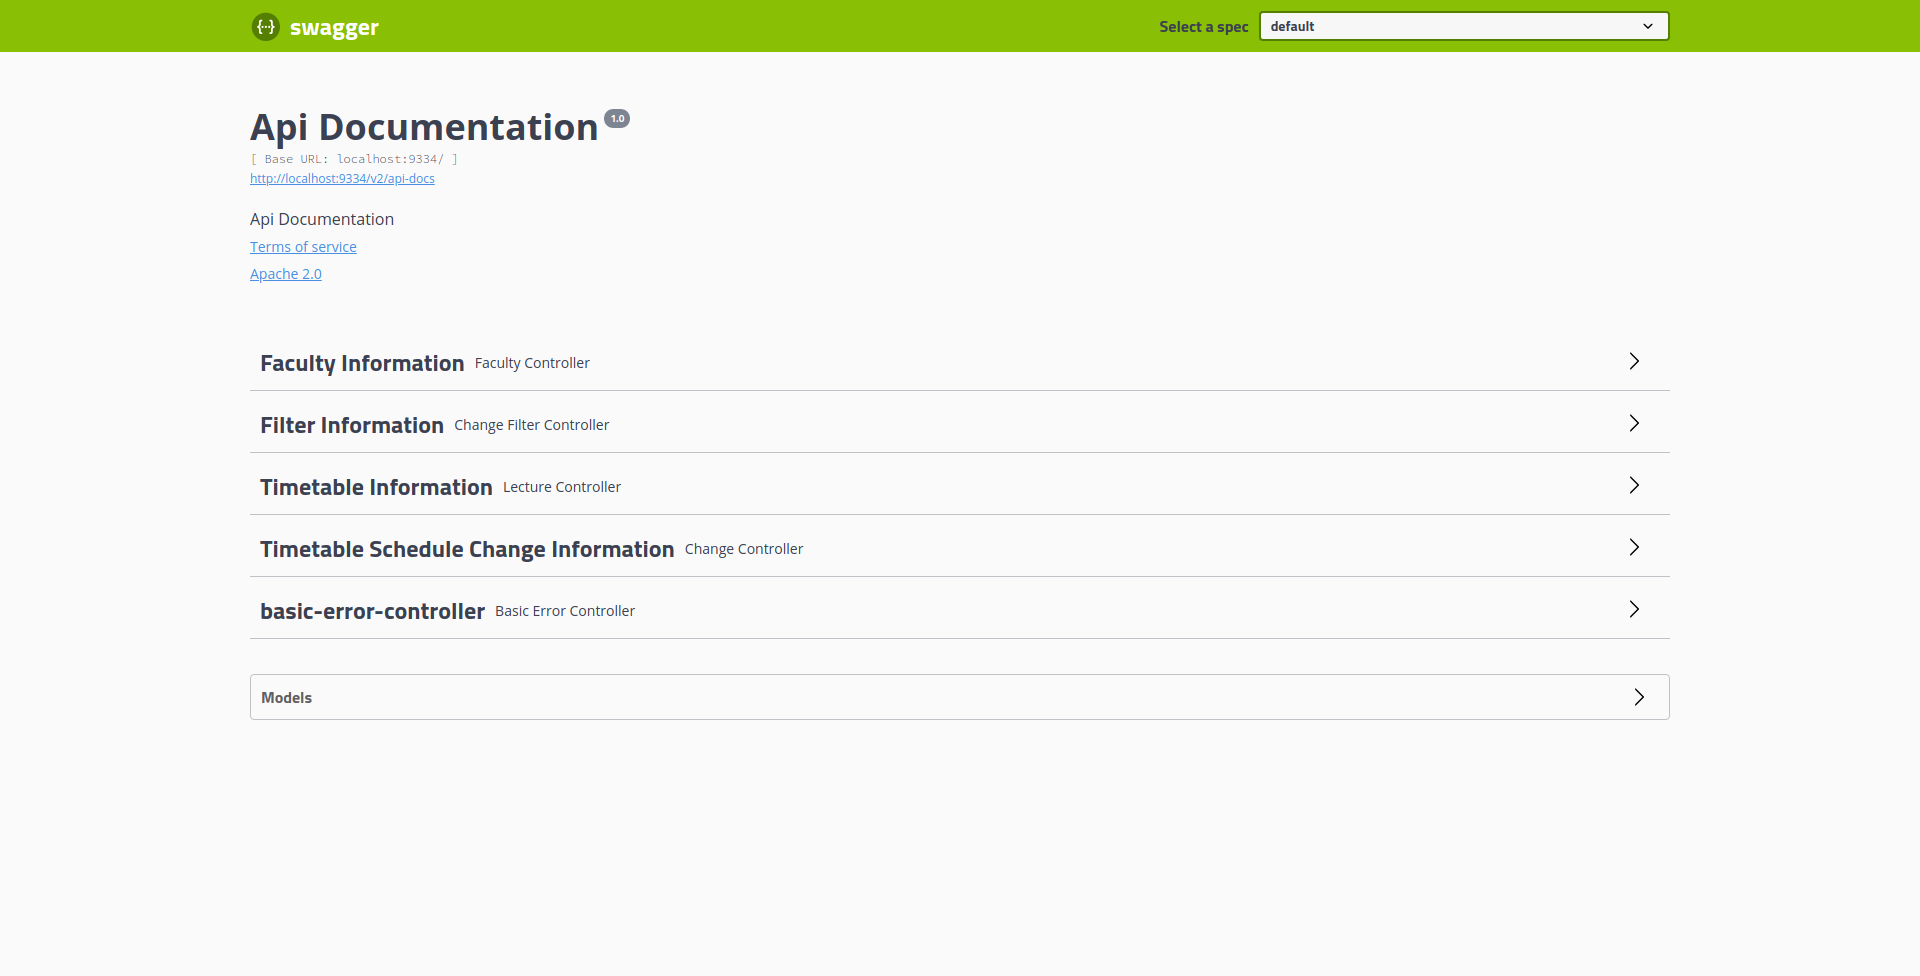
\includegraphics[width=14 cm]{Bilder/Kapitel_6/swagger_ui.png}
\caption{Swagger UI am Beispiel des Timetable-Service\label{fig:swagger_ui}}
\end{figure}

Klappt man nun eines der Controller Felder auf, so werden alle in diesem Controller verfügbaren Methoden und Endpunkte mitsamt ihrer Beschreibungen und \acp{URL} aufgelistet.

\begin{figure}[H]
\centering
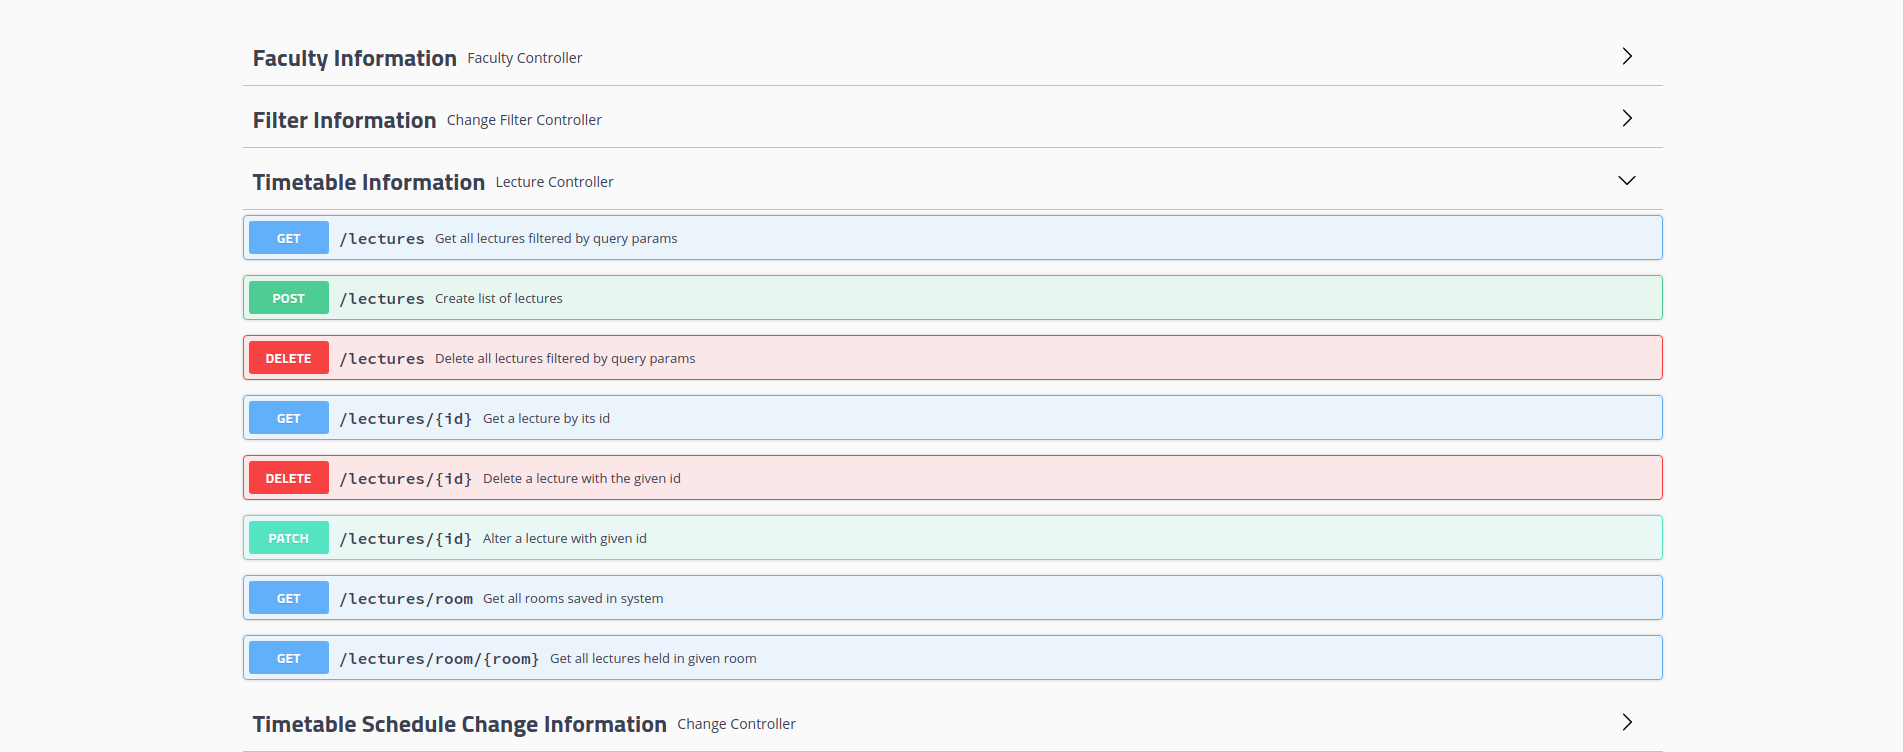
\includegraphics[width=14 cm]{Bilder/Kapitel_6/swagger_ui_methoden.png}
\caption{Swagger UI Timetable Methoden\label{fig:swagger_ui_methods}}
\end{figure}

Beim Auswählen einer der Methoden werden alle Details zu dieser einzelnen Methode angezeigt. Dazu gehören unter anderem auch alle möglichen Rückgabewerte, die Parameter, die von der Ressource akzeptiert werden und die zulässigen Werte, die in diesen Parametern übergeben werden können.

\begin{figure}[H]
\centering
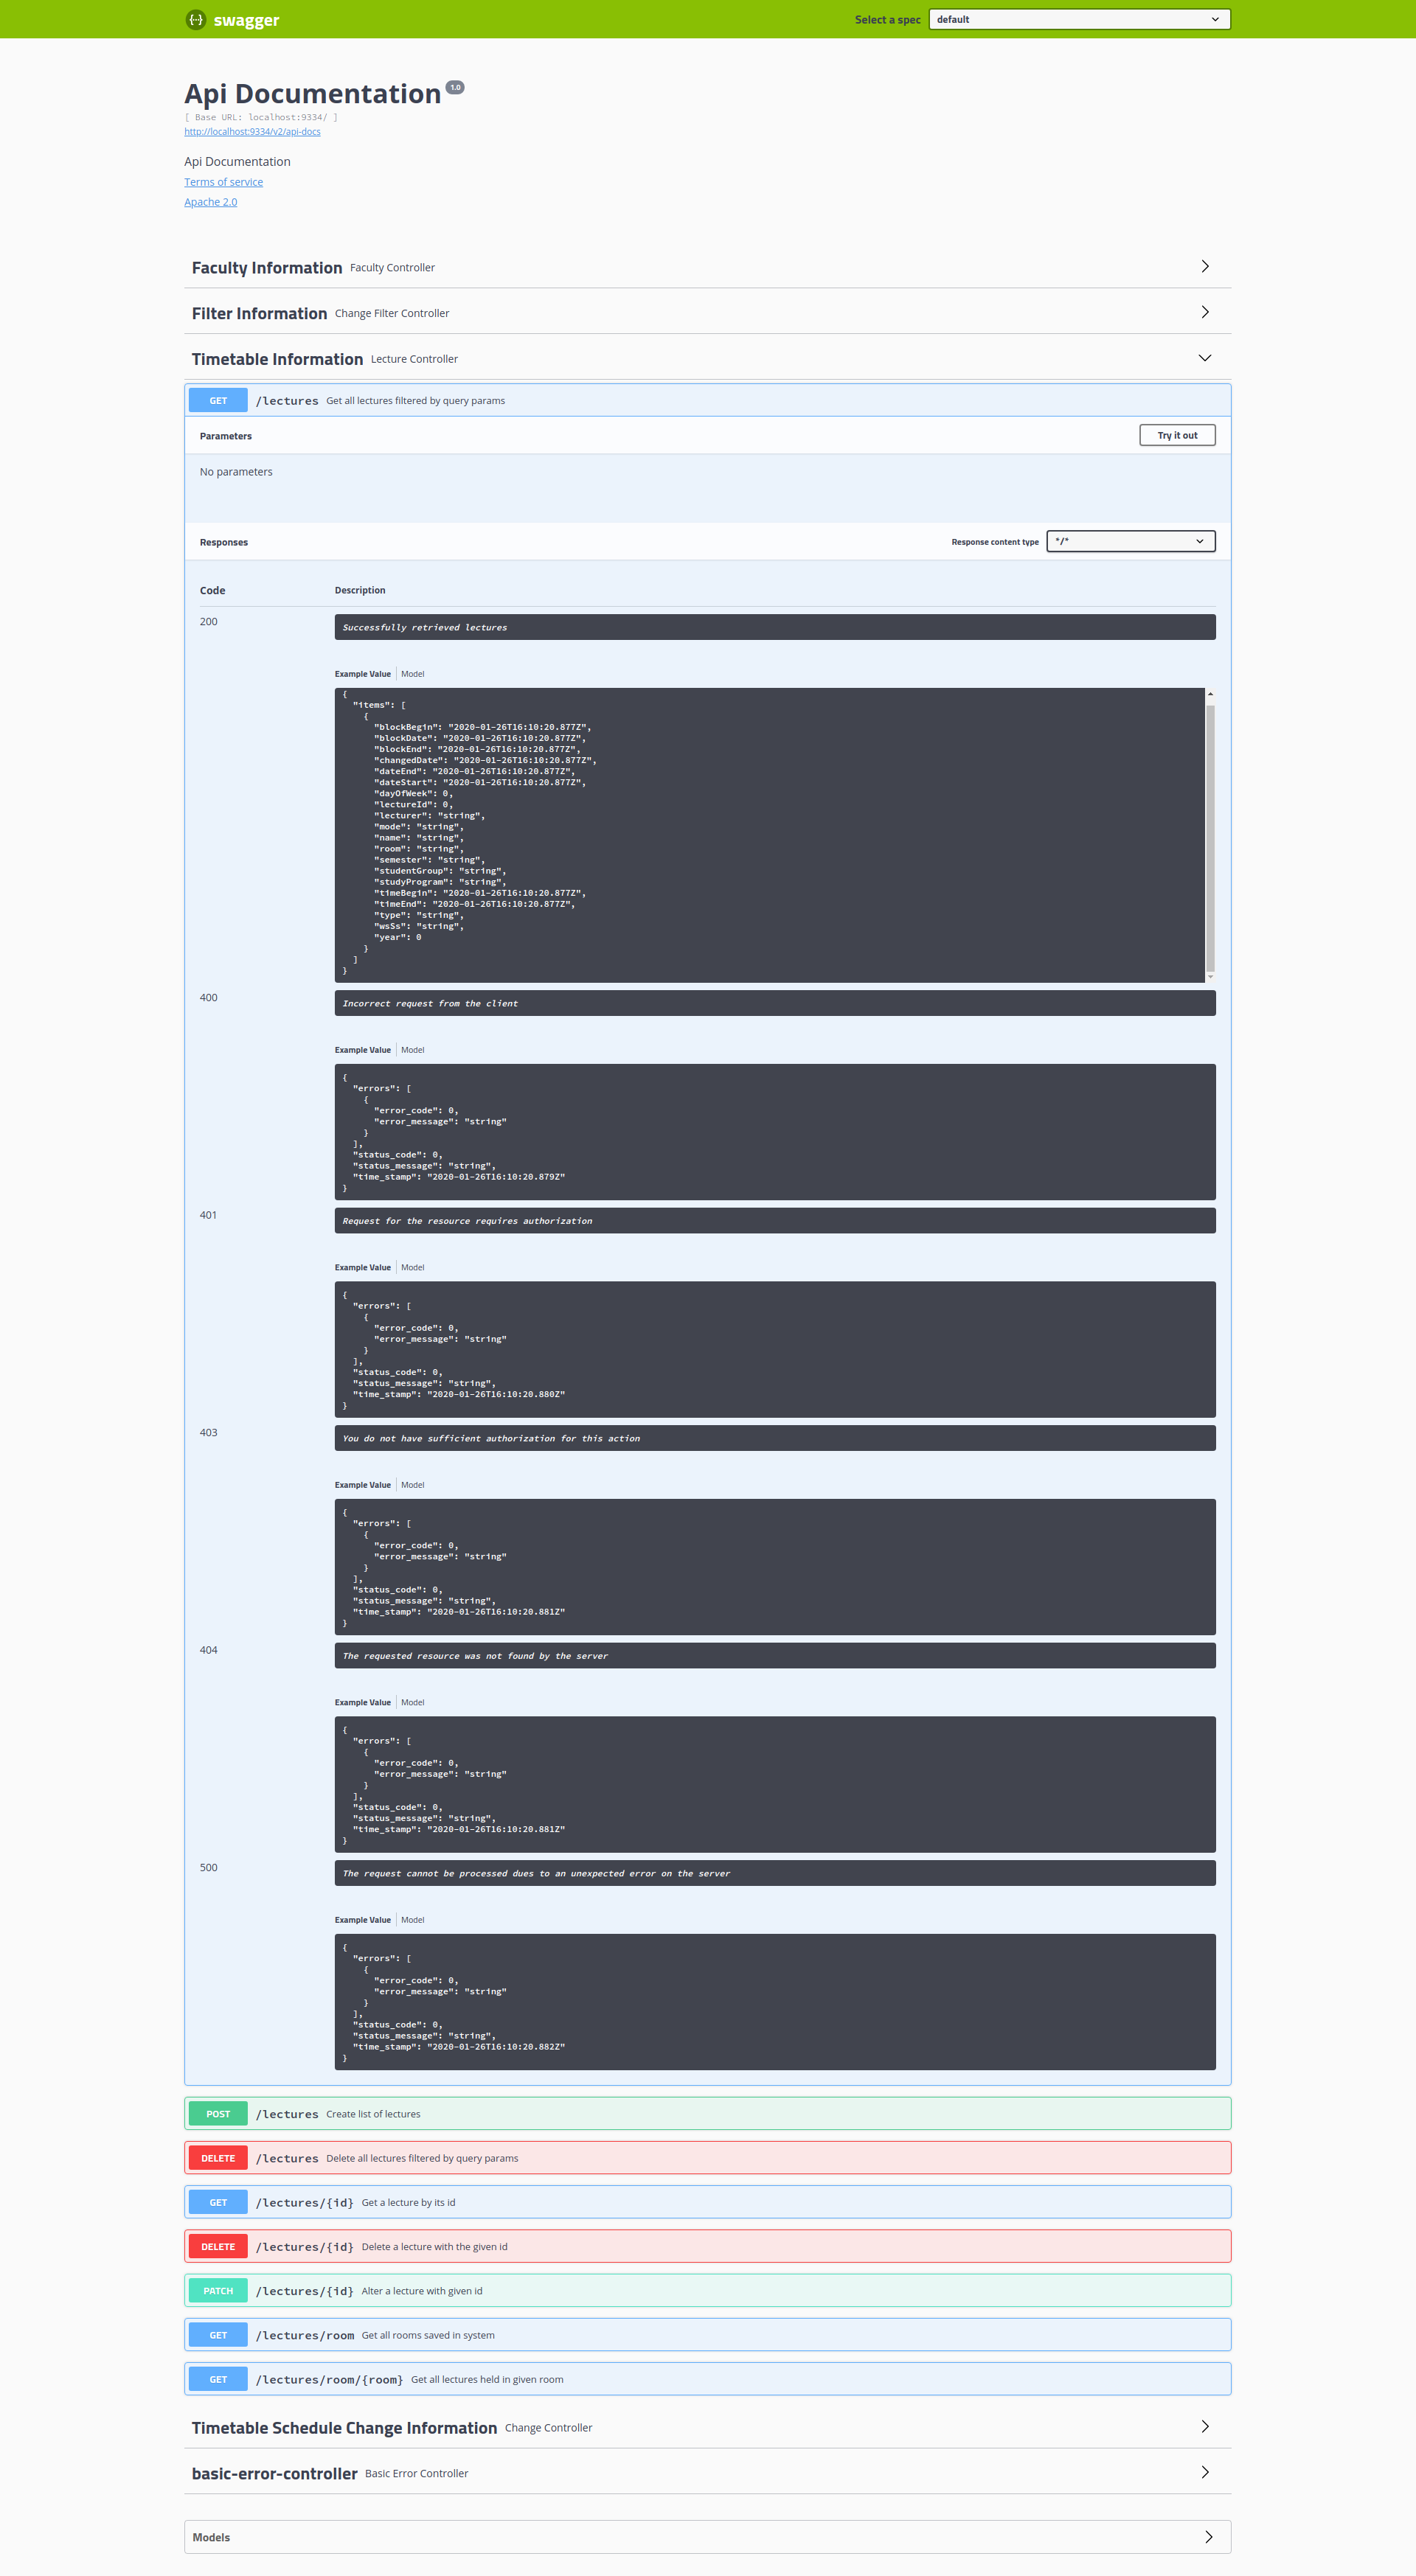
\includegraphics[width=12 cm]{Bilder/Kapitel_6/swagger_ui_method_detail.png}
\caption{Swagger UI Timetable Methoden Details\label{fig:swagger_ui_method_detail}}
\end{figure}

Wählt man nun im oberen rechten Eck der ausgewählten Ressource den Button \textit{Try it out!}, so wird dem Nutzer eine Ansicht präsentiert, die ihm die Möglichkeit gibt, alle Übergabeparameter einzugeben, die erlaubten Header für die \ac{HTTP} Anfrage zu konfigurieren und die Anfrage abzusenden. Die Anfrage wird dann an den Server weitergeleitet und ausgeführt. Hierbei ist anzumerken, dass die Anfragen unumkehrbar ausgeführt werden und nicht nur simuliert sind. Darauf präsentiert die \textit{Swagger-UI} dem Nutzer folgende Darstellung der Antwort des Servers:

\begin{figure}[H]
\centering
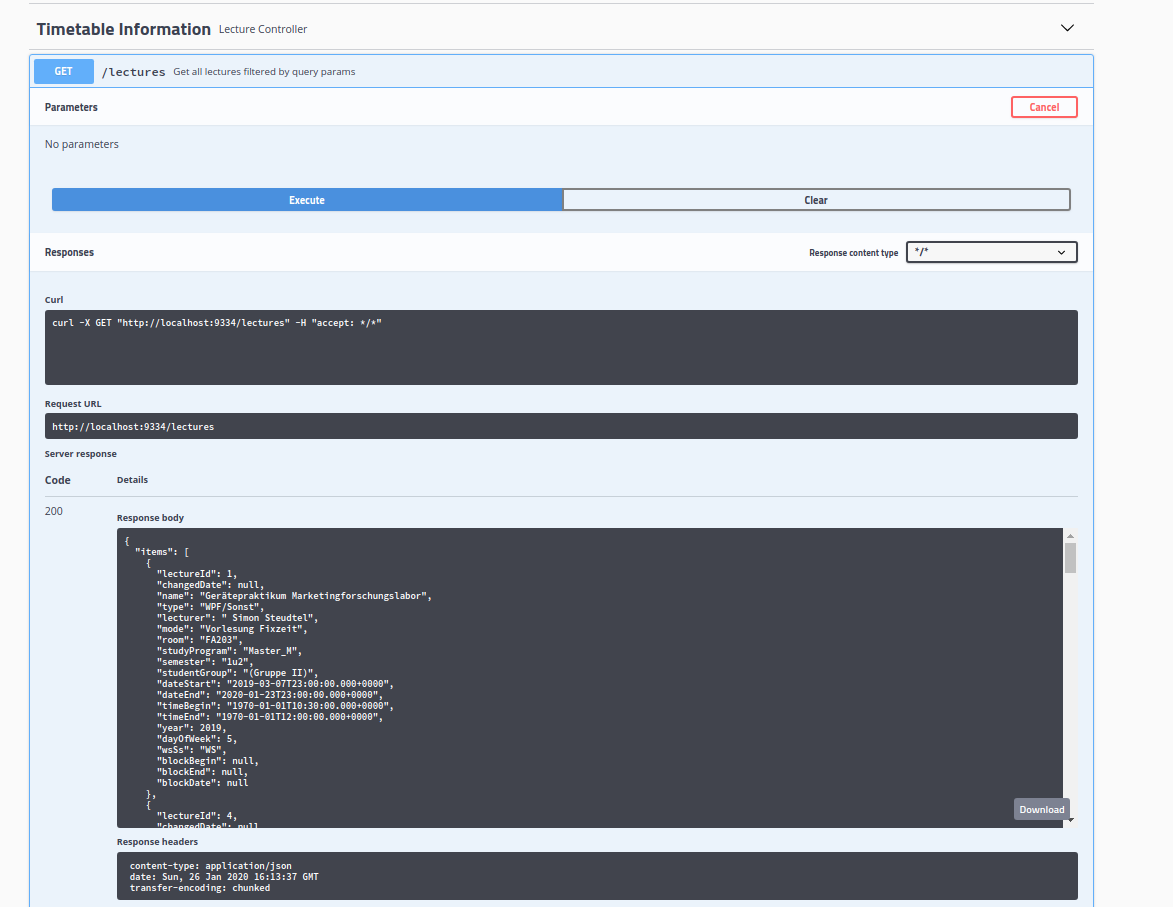
\includegraphics[width=14 cm]{Bilder/Kapitel_6/swagger_ui_try.png}
\caption{Testen einer Anfrage in der Swagger UI\label{fig:swagger_ui_try}}
\end{figure}